\documentclass[a4paper]{article}

\usepackage[portuguese]{babel}
\usepackage[utf8]{inputenc}
\usepackage[T1]{fontenc}

\newcommand{\documentTitle}{Genetic Algorithms - Brachistochrone Curve} %Macro definition
\newcommand{\documentAuthors}{João Rafael (2008111876, jprafael@student.dei.uc.pt) \and José Ribeiro (2008112181, jbaia@student.dei.uc.pt)} %Macro definition

\title{\documentTitle}
\author{\documentAuthors{}}

\usepackage{hyperref}
\hypersetup{
	pdftitle = \documentTitle
	,pdfauthor = \documentAuthors
	,pdfsubject = {Introduction to Artificial Intelligence Project \#2 Report}
	,pdfkeywords = {Artificial Intelligence Project} {Genetic Algorithms} {Brachistochrone Curve}
	,pdfborder = {0 0 0}
}

\usepackage{subfig}
\usepackage{amsmath}
\usepackage{wrapfig}
\usepackage{array}
\usepackage{anysize}
\usepackage{lscape}
\usepackage[pdftex]{graphicx}
\usepackage{longtable}
\usepackage{multirow}
\usepackage[table]{xcolor}

\marginsize{3.5cm}{3.5cm}{3cm}{3cm}

\makeatletter

\begin{document}
\renewcommand{\figurename}{Figure}
\maketitle
\cleardoublepage

\tableofcontents
\cleardoublepage

\setlength{\parindent}{1cm}
\setlength{\parskip}{0.3cm}

\section{Introduction}
\indent \indent Este projecto está inserido no âmbito da disciplina de Introdução à Inteligência Artificial,
mais concretamente no seguimento do primeiro projecto, uma vez que implementamos outro tipo de Agentes: Agentes Adaptativos.

Ao contrário dos agentes já estudados (Reactivos), estes baseiam-se fundamentalmente em conceitos da Biologia, nomeadamente a teoria da Selecção Natural de Darwin aplicada à Genética.
Estes agentes representam populações que, ao longo do tempo (iterações da aplicação), evoluem ao sofrer mutações e recombinações entre indivíduos (e os seus genes) e posterior selecção dos mais aptos.
Desta forma, pretende-se que a aptidão da população melhore, convergindo para o óptimo global.

\subsection{Brachistochrone curve}

\indent \indent O problema da curva braquistócrona é um clássico da disciplina de cálculo:

\emph{Tendo dois pontos distintos, A e B, o objectivo é conhecer a trajectória que minimiza o tempo que um ponto material demora a deslocar-se entre eles, quando sujeito apenas à força da gravidade (com atrito desprezável).}

\begin{figure}[ht]
	\centering
	\includegraphics[scale=0.5]{images/Brachistochrone.png}
	\caption{Curva Braquistócrona}
	\label{fig:brachistochrone}
\end{figure}

\indent Este problema apenas é válido quando se consideram pares de pontos com a altura de B inferior à de A, pois caso contrário o corpo não consegue efectuar o percurso.

Leibniz, L'Hospital, Newton, e os irmãos Bernoulli apresentaram soluções analíticas.
No entanto o estudo deste problema, segundo o paradigma de agentes adaptativos, é interessante pois permite calcular uma aproximação da curva
não necessitando de ferramentas matemáticas complexas.

\indent Para cada instância do problema, um indivíduo representa uma trajectória possível. Estes individuos são avaliados segundo uma
função de aptidão que mede o tempo correspondente: quanto menor, mais apto ele é considerado.

\indent De forma a definir o o formato da trajectória, cada indivíduo é caracterizado por um conjunto de genes. Estes representam os vários
factores que contribuem para a forma da trajectória, como por exemplo coordenadas, declives, curvaturas, etc. Assim, para alterar as características
de um determinado indivíduo (fenótipo) é necessário efectuar alterações ao seu conjunto genético (genótipo). Estas alterações podem se categorizar
fundamentalmente em dois tipos:

\begin{description}
	\item[Mutation] \hfill \\ 
		Alteração ou substituição de um gene por outro de origem primariamente estocástica.
	\item[Crossover] \hfill \\ 
		Aplicação de permutações no código genético de dois ou mais indivíduos, trocando a informação genética de um para outro.
\end{description}

\cleardoublepage
\section{Implementation}
\indent \indent Durante a implementação deste projecto foram surgindo abordagens alternativas,
introduzidas tanto por erros conceptuais, como por \emph{bugs}. Estas abordagens, apesar de não estarem de acordo com
o considerado comum na àrea de Inteligência Artificial, foram demonstrando capacidade de gerar soluções adequadas ao problema.
Assim, decidimos que seria interessante efectuar uma comparação entre os resultados obtidos segundo o método tradicional, e aquele a que apelidámos \emph{Rafael-Ribeiro}. 

\subsection{Representation}
\label{subsec:representation}
\indent \indent À semelhança de outros problemas\footnote[1]{Aplicação do método do trapézio para o cálculo do integral de uma curva.}, a discretização do espaço contínuo em amostras
distintas facilita a computação numérica dos resultados. Desta forma escolhemos implementar duas formas de representação:

\begin{description}
	\item[Fixed] \hfill \\
	\label{it:fixed_representation}
		Onde a curva é aproximada por um conjunto sucessivo de segmentos de recta, definidos por pares de pontos equidistantes.
	\item[Dynamic] \hfill \\
	\label{it:dynamic_representation}
		Uma representação da mesma natureza que a anterior, apenas retirando a restrição da distância entre pontos.
\end{description}

\indent Estas duas representações foram escolhidas por serem compactas, i.e.: para cada gene apenas é necessário guardar a informação das suas coordenadas.
Note-se que no caso da representação fixa a absissa é conhecida \emph{a priori}, reduzindo assim o espaço de procura exponencialmente (em relação à dinâmica).

\indent Para além destas duas representações considerámos ainda uma terceira:

\begin{description}
	\item[NURBS] \hfill \\ 
		A curva aproximada é definida à custa dos pontos de controlo de uma NURBS\footnote[2]{Non-uniform rational basis spline.}. 
		\begin{figure}[ht]
			\centering
			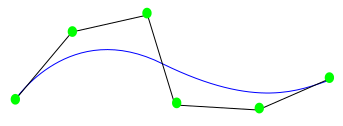
\includegraphics[scale=0.50]{images/NURBstatic.png}
			\caption{Exemplo de uma NURBS}
			\label{fig:nurbs}
		\end{figure}
\end{description}

\indent A principal vantagem desta representação é o facto de se basear em polinómios de grau superior a um, o que permite aproximar a curva desejada
com igual rigor utilizando um conjunto de pontos inferior. Desta forma o espaço de procura é mais reduzido, pelo que a convergência do algoritmo
seria esperadamente mais rápida.

\indent No entanto esta representação também apresenta os seus problemas: a avaliação da aptidão de um indivíduo depende do cálculo da derivada
desta curva, o que representa por si só um problema merecedor de uma análise profunda. 

\cleardoublepage
\subsection{Mutation Operators}
\indent \indent Um dos principais factores que contribuem para a performance de um algoritmo genético é a diversidade genética presente na população.
Desta forma, desenvolver os operadores de mutação adequados para cada problema torna-se uma tarefa crucial.
Estes actuam ao nível de cada gene e são portanto distintos para cada representação. 

\subsubsection{Fixed Representation}
\indent \indent Nesta representação o único parâmetro que se altera são as coordenadas \emph{yy} de cada gene.
Para sortear o novo valor a atribuir foi utilizada uma distribuição gaussiana (ao invés de uniforme), com o intuito 
de garantir que a evolução progenitor-filho é efectuada de forma gradual (i.e.: que o filho preserva algumas características dos
seus antecessores).

\subsubsection{Dynamic Representation}
\indent \indent Ao contrário da representação anterior, o operador de mutação para a representação dinâmica necessíta de considerar
tanto as coordenadas \emph{yy} como as \emph{xx}. Pelas razões já enunciadas, a distribuição utilizada foi novamente a gaussiana.
No entanto, uma vez que esta permite alterar a posição relativa dos pontos, é necessário efectuar um ordenamento posterior.

\indent Como estes operadores se aplicam a genes individualmente, é necessário escolher quais genes sofrem mutação.
O operador tradicional aplica uma igual probabilidade a cada gene. No entanto, segundo o paradigma biológico,
a probabilidade de erros consecutivos é mais elevada (pois a anomalia que levou à criação do primeiro erro pode ainda verificar-se).
Como achamos que esta abordagem poderia ser vantajosa para o problema em questão, decidimos implementar dois modelos de mutações adicionais:

\begin{description}
	\item[Burst] \hfill \\ 
		Onde indicamos a probabilidade de um gene ser mutado após o seu antecessor também o ser.

	\item[Partial] \hfill \\
		\label{it:partial_mutation}
		Onde por cada indivíduo são selecionados um número fixo de genes para sofer mutação.
		Este tipo de mutação é apenas aplicado para o tipo de selecção \emph{Rafael-Ribeiro}.
\end{description}
 
\cleardoublepage
\subsection{Crossover Operator}
\indent \indent O operador de recombinação distingue-se do operador de mutação na forma como tem impacto no material genético da população.
Enquanto que o operador de mutação actua sobre um único indivíduo (o que introduz novo material genético na população),
o operador de recombinação reorganiza o material genético já existente, conseguindo propagar as características entre indivíduos.
Este operador aliado a um tipo de selecção adequado (ver \ref{subsec:selection}) permite uma melhor convergência
do algoritmo.

\subsubsection{Fixed Representation}
\indent \indent Nesta representação, após o sorteio do número de pontos de recombinação (que não excede um máximo estabelecido) o operador
sorteia as coordenadas em que tais pontos de recombinação se vão aplicar, efectuando as trocas correspondentes.

\subsubsection{Dynamic Representation}
\indent \indent Dada a natureza da representação, as coordenadas sorteadas para pontos de recombinação não \emph{têm} que necessariamente existir no indivíduo.
Como tal, as coordenadas entre cada ponto de recombinação são trocadas entre si, independentemente deste processo recombinar mais ou menos genes.
Após este processo, é aplicado sobre os indivíduos com maior número de pontos (que o valor pré-definido) o operador de remoção de genes; sobre os indivíduos com menor
número de pontos é aplicado o operador de interpolação de pontos, por forma a perfazer o total de pontos do indivíduo.

\cleardoublepage
\subsection{Selection}
\label{subsec:selection}
\indent \indent Após a criação de novos descendentes é necessário efectuar uma redução no número de indivíduos.
Desta forma é possível garantir que o tamanho da população continua computacionalmente tratável e que o algoritmo convirja tendencialmente para o óptimo global.

\indent De notar que o elitismo é usualmente utilizado (excepto na selecção Rafael-Ribeiro) simultaneamente com selecção por roleta ou torneio.

\begin{description}
	\item[Elitism] \hfill \\
		Abordagem gananciosa que seleciona os melhores indivíduos da população como descendetes.

	\item[Roulette] \hfill \\
		Os indivíduos são selecionados de forma aleatória, dando maior probabilidade aos indivíduos com maior fitness.
		Para garantir esta propriedade a função de probabilidade para um indivíduo $i$ é:

		\[
			p_{i} = \frac{f_{i}}{\sum\limits_{j \in \text{Pop.}} f_{j}} \quad \text{onde} \quad f_i = \frac{1}{T_{i}} \quad (T_{i} \leftarrow \text{Tempo correspondente ao indivíduo } i)
		\]

		Neste algoritmo o mesmo elemento pode ser escolhido várias vezes,
		simulando a capacidade de um ser mais apto se conseguir reproduzir com maior frequência.

	\item[Tournament] \hfill \\ 
		Para este tipo de selecção são escolhidos aleatoriamente N indivíduos, dos quais apenas o mais apto é escolhido.
		Após esta selecção todos os elementos participantes no torneio são devolvidos à população.

	\item[Rafael-Ribeiro] \hfill \\
		Nesta abordagem implementa-se em conjunto a selecção por elitismo e por torneio, mas ao contrário da abordagem tradicional
		esta é aplicada não só para selecionar os progenitores, mas também para selecionar que indivíduos da população inteira (pais e filhos)
		sobrevivem para a próxima iteração. Do ponto de vista que apenas alguns indivíduos são alterados, este tipo de selecção pode ser considerada \emph{Steady-State}.

\end{description}

\cleardoublepage

\section{Experiments}
\label{sec:experiments}
\indent \indent Os resultados obtidos com algoritmos genéticos dependem intrinsecamente dos parâmetros com os quais são executados
(representação, modo de selecção, percentagem de elitismo, ...). Assim, para uma correcta análise do seu comportamento
torna-se necessário analisar as várias combinações. Como tal, para cada parâmetro foram escolhidos 2 ou 3 valores.
Enumeram-se de seguida as variações.

\begin{description}
	\item [Points set] \hfill \\
		\indent Foram utilizados dois conjuntos de pontos (inicial e final) para averiguar a correcta convergência em diferentes casos.
			\begin{description}
				\item \[ P_{init} = (0.0, 3.0),\quad P_{final} = (4.0, 2.0) \]
				\item \[ P_{init} = (0.0, 3.0),\quad P_{final} = (4.0, 2.8) \]
			\end{description}
	\item [Representation] \hfill \\
		\indent Foram testados os tipos de representação já mencionados em \ref{subsec:representation}.
	\item [Selection] \hfill \\
		\indent Foram testados os tipos de selecção já mencionados em \ref{subsec:selection}. No entanto, o elitismo foi variado em simultâneo com
		as selecções Torneio, Roleta e Rafael-Ribeiro, uma vez que são aplicadas em fases diferentes do algoritmo.
	\begin{description}
		\item [Elitismo] \hfill \\
			\indent Os valores utilizados foram 5\% e 20\%. Pensamos que 5\% é um valor adequado dado o contexto do problema; 20\%
			foi escolhido para averiguar se a convergência do algoritmo para um óptimo global ainda se manteria.
	\end{description}
	\item [No. of points] \hfill \\
		\indent Os valores utilizados para o número de pontos foram 15 e 30; estes valores foram escolhidos após experimentação, dado que concluímos
		que um maior número de pontos torna o espaço de procura demasiado extenso.
	\item [Population size] \hfill \\
		\indent Para os tamanhos de população foram utilizados os valores de 25, 50 e 100 indivíduos. %TODO Justificar como sendo valores adequados (após experimentação)?
	\item [Crossover probability] \hfill \\
		\indent Para a probabilidade de ocorrência de recombinação foram escolhidos os valores de 0\% e 35\%. A escolha do valor de 35\% ocorreu após
		experimentação; já o valor de 0\% foi escolhido para testar os resultados em que a única variação/propagação do material genético da população se deve
		a mutações aliadas a métodos de selecção. De notar que quando a probabilidade de recombinação é 0\% o parâmetro relativo ao número de pontos de recombinação
		não é aplicado.
	\item [Crossover points] \hfill \\
		\indent Os dois valores de pontos de recombinação utilizados foram 2 e 5. %TODO Existe justificação?
	\item [Mutation probability] \hfill \\
		\indent Os valores utilizados para a probabilidade de mutação foram 5\% e 25\%. %TODO Existe justificação?
\end{description}

\cleardoublepage

\section{Validation}
\indent \indent Para validar o comportamento do Agente, cada combinação de parâmetros foi executada 30 vezes com seeds diferentes;
tal garante que a natureza estocástica do algoritmo fica evidenciada ao garantir que os testes são, de facto, diferentes.

Após a conclusão dos testes, foi calculado o desvio-padrão entre as 30 simulações,
para averiguar se os resultados obtidos não representavam apenas um caso de sorte.

Tal como se pode verificar na última coluna da tabela de resultados (Secção \ref{tab:results}), o desvio-padrão entre as 30 simulações para cada combinação de parâmetros
é bastante reduzido\footnote[1]{São excepção os testes onde a probabilidade de recombinação é 0.00\%, pois a ausência deste operador torna a evolução individual,
não tomando partido das soluções obtidas pelos outros indivíduos da população.}, o que comprova a sua consistência e robustez.

\cleardoublepage
\section{Result Analysis}

\cleardoublepage
\subsection{Representation}
\begin{figure}[ht]
	\centering
	\subfloat[200 iterations]{\includegraphics[width=0.3\textwidth]{images/evolution_200.png}}
	\subfloat[2000 iterations]{\includegraphics[width=0.3\textwidth]{images/evolution_2000.png}}
	\subfloat[5000 iterations]{\includegraphics[width=0.3\textwidth]{images/evolution_5000.png}}
	\caption{Fitness evolution}
\end{figure}

\indent \indent Como é possível observar pelos gráficos (ou constatar nas tabelas da secção \ref{sec:fitness_by_representation}), a representação fixa converge mais rapidamente para o óptimo global
(permitido por esta) do que a representação dinâmica. Esta propriedade justifica-se pelo facto do espaço de procura ser
mais reduzido. No entanto, por essa mesma razão, o valor final de aptidão obtido é inferior ao obtido com a representação dinâmica.
O número de iterações a partir do qual compensa utilizar uma representação dinâmica depende do número de pontos utilizado, bem como dos pontos iniciais e finais.

\indent Outra propriedade merecedora de análise é a média das aptidões dos melhores indíviduos para cada representação.
Como podemos observar na tabela correspondente \ref{sec:fitness_by_representation}, a média é inferior para a representação igualmente espaçada,
o que nos indica que esta é mais consistente (i.e.: menos sensível a ajustes de parâmetros). 

\cleardoublepage

\subsection{Selection}
\indent \indent Como é possível verificar na tabela da secção \ref{sec:fitness_by_selection}, a "selecção"\footnote[1]{De relembrar o leitor de que o algoritmo Rafael-Ribeiro
apresenta um funcionamento diferente ao nível das mutações, não sendo assim classificável como puramente um método de selecção.} Rafael-Ribeiro é claramente
superior na representação de pontos igualmente espaçados. Tal deve-se à sua abordagem semelhante a Estado Estável, isto é, estocasticamente a percentagem de
indivíduos de elevada aptidão que permanece na geração seguinte é superior; este facto favorece o tipo de mutação utilizado (ver secção \ref{it:partial_mutation}),
o que força uma melhor convergência do algoritmo ao permitir fugas de óptimos locais.

\indent Na mesma tabela da secção \ref{sec:fitness_by_selection} é possível observar que a representação dinamicamente espaçada obtém melhores resultados com a Roleta.
Tal se deve ao facto de o seu espaço de procura ser exponencialmente maior do que o da representação igualmente espaçada. Assim, a Roleta ao favorecer a diversidade
genética permite uma melhor exploração do espaço de procura ao permitir que indivíduos menos bons permaneçam nas gerações seguintes.

\cleardoublepage

\subsection{Crossover}
\indent \indent Tal como indicado na secção \ref{sec:experiments} o parâmetro de recombinação a 0\% foi experimentado com o
intuito de verificar o impacto do operador de recombinação. Esta situação foi comprovada experimentalmente e pode ser observada em \ref{sec:crossover_on_off}.

\indent Por outro lado o número de pontos de recombinação utilizados demonstrou ser um factor irrelevante à performance do algoritmo.

\cleardoublepage
\subsection{Population Size}
\indent \indent Os dados presentes na tabela \ref{sec:results} indicam, tal como esperado, que quanto maior a população melhores
os resultados. No entanto, uma vez que aumentar o tamanho da população aumenta necessáriamente
o tempo de computação de cada iteração, torna-se interessante analisar mais detalhadamente este \emph{trade-off}.

\indent Como é possível observar na tabela \ref{sec:fitness_by_population_size}, os resultados obtidos com uma
população de \emph{n} indivíduos em \emph{m} iterações são ligeiramente melhores que os obtidos
com uma população com o dobro do tamanho em metade do tempo. Esta convergência mais rápida justifica-se
pelo facto de existirem menos indivíduos a seguirem caminhos evolucionários semelhantes. No entanto, por esta
mesma razão a resistência a óptimos locais é inferior.
 
\cleardoublepage

\subsection{Mutation}
\indent \indent TODO % TODO FIXME

\subsubsection{Mutation burst}
\indent \indent TODO % TODO FIXME

\cleardoublepage

\eject \pdfpagewidth=594.0mm \pdfpageheight=420.0mm
\paperwidth=594.0mm
\paperheight=420.0mm

\section{Attachments}

\subsection{Results' Table}
\label{sec:results}
\begin{center}
	\input{tables/results}
\end{center}

\eject \pdfpagewidth=210.0mm \pdfpageheight=297.0mm

\subsection{Fitness by representation}
\label{sec:fitness_by_representation}
\begin{center}
	\begin{tabular}{|c|c|c|c|c|}
		\hline
		\multirow{3}{*}{Iterations}	&	\multicolumn{4}{c|}{Best fitness by representation}																													\\
										\cline{2-5}
									&	\multicolumn{2}{c|}{Points set 1}												& \multicolumn{2}{c|}{Points set 2}													\\
										\cline{2-5}
									&	Even								&	Dynamic									&	Even									&	Dynamic								\\
		\noalign{\hrule height 1.5pt}
		20							& 1.2943594 \cellcolor[gray]{0.9}		& 1.4232276									& 1.6813473 \cellcolor[gray]{0.9}			& 1.7981805								\\
		\hline
		100							& 1.2323244	\cellcolor[gray]{0.9}		& 1.2447508									& 1.4464484	\cellcolor[gray]{0.9}			& 1.5103336								\\
		\hline
		1000						& 1.2220753 							& 1.2149932 \cellcolor[gray]{0.9}			& 1.4177439									& 1.4088078 \cellcolor[gray]{0.9}		\\
		\hline
		2000						& 1.2216504					 			& 1.2140057 \cellcolor[gray]{0.9}			& 1.4166930									& 1.4074098	\cellcolor[gray]{0.9}		\\
		\hline
	\end{tabular}
	\label{tab:representation_type_best}
\end{center}

\begin{center}
	\begin{tabular}{|c|c|c|c|c|}
		\hline
		\multirow{3}{*}{Iterations}	&	\multicolumn{4}{c|}{Bests' average fitness by representation}																\\
										\cline{2-5}
									&	\multicolumn{2}{c|}{Points set 1}							& \multicolumn{2}{c|}{Points set 2}								\\
										\cline{2-5}
									&	Even			&	Dynamic			&	Even				&	Dynamic														\\
		\noalign{\hrule height 1.5pt}
	20								&	2.0281445 \cellcolor[gray]{0.9}		&	2.2345551			&	2.1971514 \cellcolor[gray]{0.9} 		&	2.2104010		\\
	\hline
	100								&	1.4861452 \cellcolor[gray]{0.9}		&	1.7393440			&	1.8409800 \cellcolor[gray]{0.9}			&	1.8605020		\\
	\hline
	1000 							&	1.2820714 \cellcolor[gray]{0.9} 	&	1.3750536			&	1.5588395 \cellcolor[gray]{0.9}			&	1.5681385		\\
	\hline
	2000							&	1.2685988 \cellcolor[gray]{0.9} 	&	1.3238336			&	1.5234296 \cellcolor[gray]{0.9}			&	1.5245320		\\
	\hline
	\end{tabular}
	\label{tab:representation_type_best_avg}
\end{center}



\subsection{Fitness by selection}
\label{sec:fitness_by_selection}
\begin{center}
	\begin{tabular}{|c|c|c|c|c|c|c|}
		\hline
		\multirow{3}{*}{Iterations}	&	\multicolumn{6}{c|}{Points set 1 best by selection}	\\
										\cline{2-7}
									&	\multicolumn{3}{c|}{Even}																		& \multicolumn{3}{c|}{Dynamic} \\
										\cline{2-7}
									&	Tournament		&	Roulette							&	Rafael-Ribeiro						&	Tournament							&	Roulette							&	Rafael-Ribeiro		\\
		\noalign{\hrule height 1.5pt}
		20							&	1.3035679		& 	1.2943594 \cellcolor[gray]{0.9}		&	1.3855835							&	1.4306861							&	1.4232276 \cellcolor[gray]{0.9}		&	1.4422860			\\
		\hline
		100							&	1.2339894		&	1.2334137							&	1.2323244 \cellcolor[gray]{0.9}		&	1.2447508 \cellcolor[gray]{0.9} 	&	1.2462901							&	1.2509805			\\
		\hline
		1000						&	1.2260637		&	1.2257382							&	1.2220753 \cellcolor[gray]{0.9}		&	1.2152843							&	1.2149932 \cellcolor[gray]{0.9}		&	1.2154610			\\
		\hline
		2000						&	1.2249858		&	1.2248156							&	1.2216504 \cellcolor[gray]{0.9}		&	1.2140487							&	1.2140057 \cellcolor[gray]{0.9}		&	1.2143019			\\
		\hline
	\end{tabular}
	\label{tab:selection_type_1_best}
\end{center}

\begin{center}
	\begin{tabular}{|c|c|c|c|c|c|c|}
		\hline
		\multirow{3}{*}{Iterations}	&	\multicolumn{6}{c|}{Points set 1 bests' average by selection}	\\
										\cline{2-7}
									&	\multicolumn{3}{c|}{Even}																							& \multicolumn{3}{c|}{Dynamic} \\
										\cline{2-7}
									&	Tournament							&	Roulette							&	Rafael-Ribeiro						&	Tournament		&	Roulette							&	Rafael-Ribeiro		\\
		\noalign{\hrule height 1.5pt}
		20							&	1.9092792 \cellcolor[gray]{0.9}		&	1.9141063							&	2.2610480							&	2.2027320		&	2.2022573 \cellcolor[gray]{0.9}		&	2.2986759			\\
		\hline
		100							&	1.4300238 \cellcolor[gray]{0.9}		&	1.4328046							&	1.5956073							&	1.7007847		&	1.6934133 \cellcolor[gray]{0.9}		&	1.8238340			\\
		\hline
		1000						&	1.2973567							&	1.2972244 \cellcolor[gray]{0.9}		&	1.2516332							&	1.3568962		&	1.3556743 \cellcolor[gray]{0.9}		&	1.4125902			\\
		\hline
		2000						&	1.2830978							&	1.2831009							&	1.2395977 \cellcolor[gray]{0.9}		&	1.3076324		&	1.3072849 \cellcolor[gray]{0.9}		&	1.3565834			\\
		\hline
	\end{tabular}
	\label{tab:selection_type_1_avg}
\end{center}

\begin{center}
	\begin{tabular}{|c|c|c|c|c|c|c|}
		\hline
		\multirow{3}{*}{Iterations}	&	\multicolumn{6}{c|}{Points set 2 best by selection}	\\
										\cline{2-7}
									&	\multicolumn{3}{c|}{Even}																							& \multicolumn{3}{c|}{Dynamic} \\
										\cline{2-7}
									&	Tournament							&	Roulette							&	Rafael-Ribeiro						&	Tournament							&	Roulette							&	Rafael-Ribeiro		\\
		\noalign{\hrule height 1.5pt}
		20							&	1.6924473							&	1.6813473 \cellcolor[gray]{0.9}		&	1.8119261							&	1.7981805 \cellcolor[gray]{0.9}		&	1.8119160							&	1.8417157			\\
		\hline
		100							&	1.4471459							&	1.4464484 \cellcolor[gray]{0.9}		&	1.4959512							&	1.5140132							&	1.5103336 \cellcolor[gray]{0.9}		&	1.5278036			\\
		\hline
		1000						&	1.4208745 \cellcolor[gray]{0.9}		&	1.4209846							&	1.4177439							&	1.4094479							&	1.4093918							&	1.4088078 \cellcolor[gray]{0.9}			\\
		\hline	
		2000						&	1.4195882							&	1.4198324							&	1.4166930 \cellcolor[gray]{0.9}		&	1.4074098 \cellcolor[gray]{0.9}		&	1.4074232							&	1.4074721			\\
		\hline
	\end{tabular}
	\label{tab:selection_type_2_best}
\end{center}

\begin{center}
	\begin{tabular}{|c|c|c|c|c|c|c|}
		\hline
		\multirow{3}{*}{Iterations}	&	\multicolumn{6}{c|}{Points set 2 bests' average by selection}	\\
										\cline{2-7}
									&	\multicolumn{3}{c|}{Even}													& \multicolumn{3}{c|}{Dynamic} \\
										\cline{2-7}
									&	Tournament		&	Roulette		&	Rafael-Ribeiro						&	Tournament							&	Roulette							&	Rafael-Ribeiro		\\
		\noalign{\hrule height 1.5pt}
		20 							&	2.2044574		&	2.2046092		&	2.1823877 \cellcolor[gray]{0.9}		&	2.1948890 \cellcolor[gray]{0.9}		&	2.2007685							&	2.2355455			\\
		\hline
		100							&	1.8496719		&	1.8502629		&	1.8230053 \cellcolor[gray]{0.9}		&	1.8435026							&	1.8432013 \cellcolor[gray]{0.9}		&	1.8948020			\\	
		\hline
		1000						&	1.5668211		&	1.5687835		&	1.5409138 \cellcolor[gray]{0.9}		&	1.5646693							&	1.5637325 \cellcolor[gray]{0.9}		&	1.5760138			\\
		\hline
		2000						&	1.5322085		&	1.5333797		&	1.5047007 \cellcolor[gray]{0.9}		&	1.5226141							&	1.5219615 \cellcolor[gray]{0.9}		&	1.5290204			\\
		\hline
	\end{tabular}
	\label{tab:selection_type_2_avg}
\end{center}




\subsection{Fitness by population size}
\label{sec:fitness_by_population_size}
\begin{center}
	\begin{tabular}{rr!{\vrule width 1.5pt}c|c!{\vrule width 1.5pt}c|c}
															\cline{2-6}
		\multicolumn{1}{r}{\multirow{2}{*}{}} 					& \multicolumn{1}{|r!{\vrule width 1.5pt}}{Population size} 	& 25 		& 50		& 50 		& \multicolumn{1}{c|}{100} 	\\
																\cline{2-6}
																& \multicolumn{1}{|r!{\vrule width 1.5pt}}{Iteration} 			& 2000		& 1000		& 2000 		& \multicolumn{1}{c|}{1000} 	\\
		\hline		
		\multicolumn{1}{|r}{\multirow{2}{*}{Representation}}	& \multicolumn{1}{|r!{\vrule width 1.5pt}}{Fixed}				& NA 		& NA		& NA 		& \multicolumn{1}{c|}{NA} 	\\
																\cline{2-6}
		\multicolumn{1}{|r}{}									& \multicolumn{1}{|r!{\vrule width 1.5pt}}{Dynamic}				& NA 		& NA		& NA 		& \multicolumn{1}{c|}{NA} 	\\
	\hline
	\end{tabular}
	\captionof{table}{Comparison between population sizes}
	\label{tab:population_size_best_avg}
\end{center}



\subsection{With and Without Crossover}
\label{sec:crossover_on_off}
\begin{center}
	\begin{tabular}{|c|c|c|c|c|}
		\hline
		\multicolumn{1}{|c|}{\multirow{3}{*}{Iterations}} 	& \multicolumn{4}{c|}{ Representation }\\
															\cline{2-5}
															& \multicolumn{2}{c|}{ Fixed } 							& \multicolumn{2}{c|}{ Dynamic } \\
															\cline{2-5}
		 													& 0\% 		& 35\% 										& 0\% 								& 35\% 									\\
		\noalign{\hrule height 1.5pt}
		20 													& 2.1585019	& 1.9629658	\cellcolor[gray]{0.9}			& 2.2329140 \cellcolor[gray]{0.9} 	& 2.2353757 							\\
		\hline
		100 												& 1.5264924 & 1.4659716	\cellcolor[gray]{0.9}			& 1.7353239 \cellcolor[gray]{0.9} 	& 1.7413541 							\\
		\hline
		1000 												& 1.2842884 & 1.2809630	\cellcolor[gray]{0.9}			& 1.3779161 						& 1.3736223 \cellcolor[gray]{0.9} 		\\
		\hline
		2000 												& 1.2700742 & 1.2678611	\cellcolor[gray]{0.9}			& 1.3254627 						& 1.3230190 \cellcolor[gray]{0.9}		\\
		\hline
	\end{tabular}
	\captionof{table}{Crossover impact}
	\label{tab:crossover_on_off}
\end{center}



\subsection{Crossover points}
\label{sec:crossover_points}
\begin{center}
	\begin{tabular}{|c|c|c|}
	\hline
		\multicolumn{1}{|c|}{\multirow{2}{*}{Iterations}} 	& \multicolumn{2}{c|}{Number of cross points} 	\\
														\cline{2-3}
		 												& 2 			& 5 							\\
	\noalign{\hrule height 1.5pt}
		20 												& 1.7146707 	& 1.7095787 					\\
	\hline
		100 											& 1.4019046 	& 1.3998350 					\\
	\hline
		1000 											& 1.2621355 	& 1.2624915						\\
	\hline
		2000 											& 1.2568907 	& 1.2568924						\\
	\hline
	\end{tabular}
	\captionof{table}{Comparison between crossover with 2 and 5 points}
	\label{tab:crossover_points}
\end{center}


\subsection{Mutation}
\label{sec:mutation}
\input{tables/mutation}

\subsection{Mutation Burst}
\label{sec:mutation_burst}
\begin{center}
	\begin{tabular}{|c|c|c|c|c|}
		\hline
		\multicolumn{1}{|c|}{\multirow{3}{*}{Iterations}} 	& \multicolumn{4}{c|}{ Representation }\\
															\cline{2-5}
															& \multicolumn{2}{c|}{ Fixed } 							& \multicolumn{2}{c|}{ Dynamic } \\
															\cline{2-5}
		 													& 0\% 		& 35\% 										& 0\% 								& 35\% 	\\
		\noalign{\hrule height 1.5pt}
		20 													& 			& 											& 									& 		\\
		\hline
		100 												& 			& 											& 									&  		\\
		\hline
		1000 												&  			& 											& 									&  		\\
		\hline
		2000 												&  			& 											& 									&  		\\
		\hline
	\end{tabular}
	\captionof{table}{Mutation burst impact; for fixed representation tournament selection was used since Rafael-Ribeiro doesn't allow for bursts}
	\label{tab:mutation_burst}
\end{center}



\end{document}
